% Copyright 2020 Glen Newton
% License: Creative Commons Attribution-ShareAlike 4.0 International License https://creativecommons.org/licenses/by-sa/4.0/legalcode
\documentclass[12pt]{article}
\usepackage{tikz}

\usepackage[extreme]{savetrees}
\usepackage{microtype}
\usepackage[hidelinks]{hyperref}
\usetikzlibrary{mindmap,positioning}

%\usepackage{atbegshi}% http://ctan.org/pkg/atbegshi
%\AtBeginDocument{\AtBeginShipoutNext{\AtBeginShipoutDiscard}}


% from: https://tex.stackexchange.com/questions/250150/formatting-mindmap-in-tikz
\hypersetup{
  colorlinks=false
  }

% from: https://tex.stackexchange.com/questions/107057/adjusting-font-size-with-tikz-picture

\begin{document}
\sffamily
\pagestyle{empty}
          {\centering
            \makebox[0pt]{%
              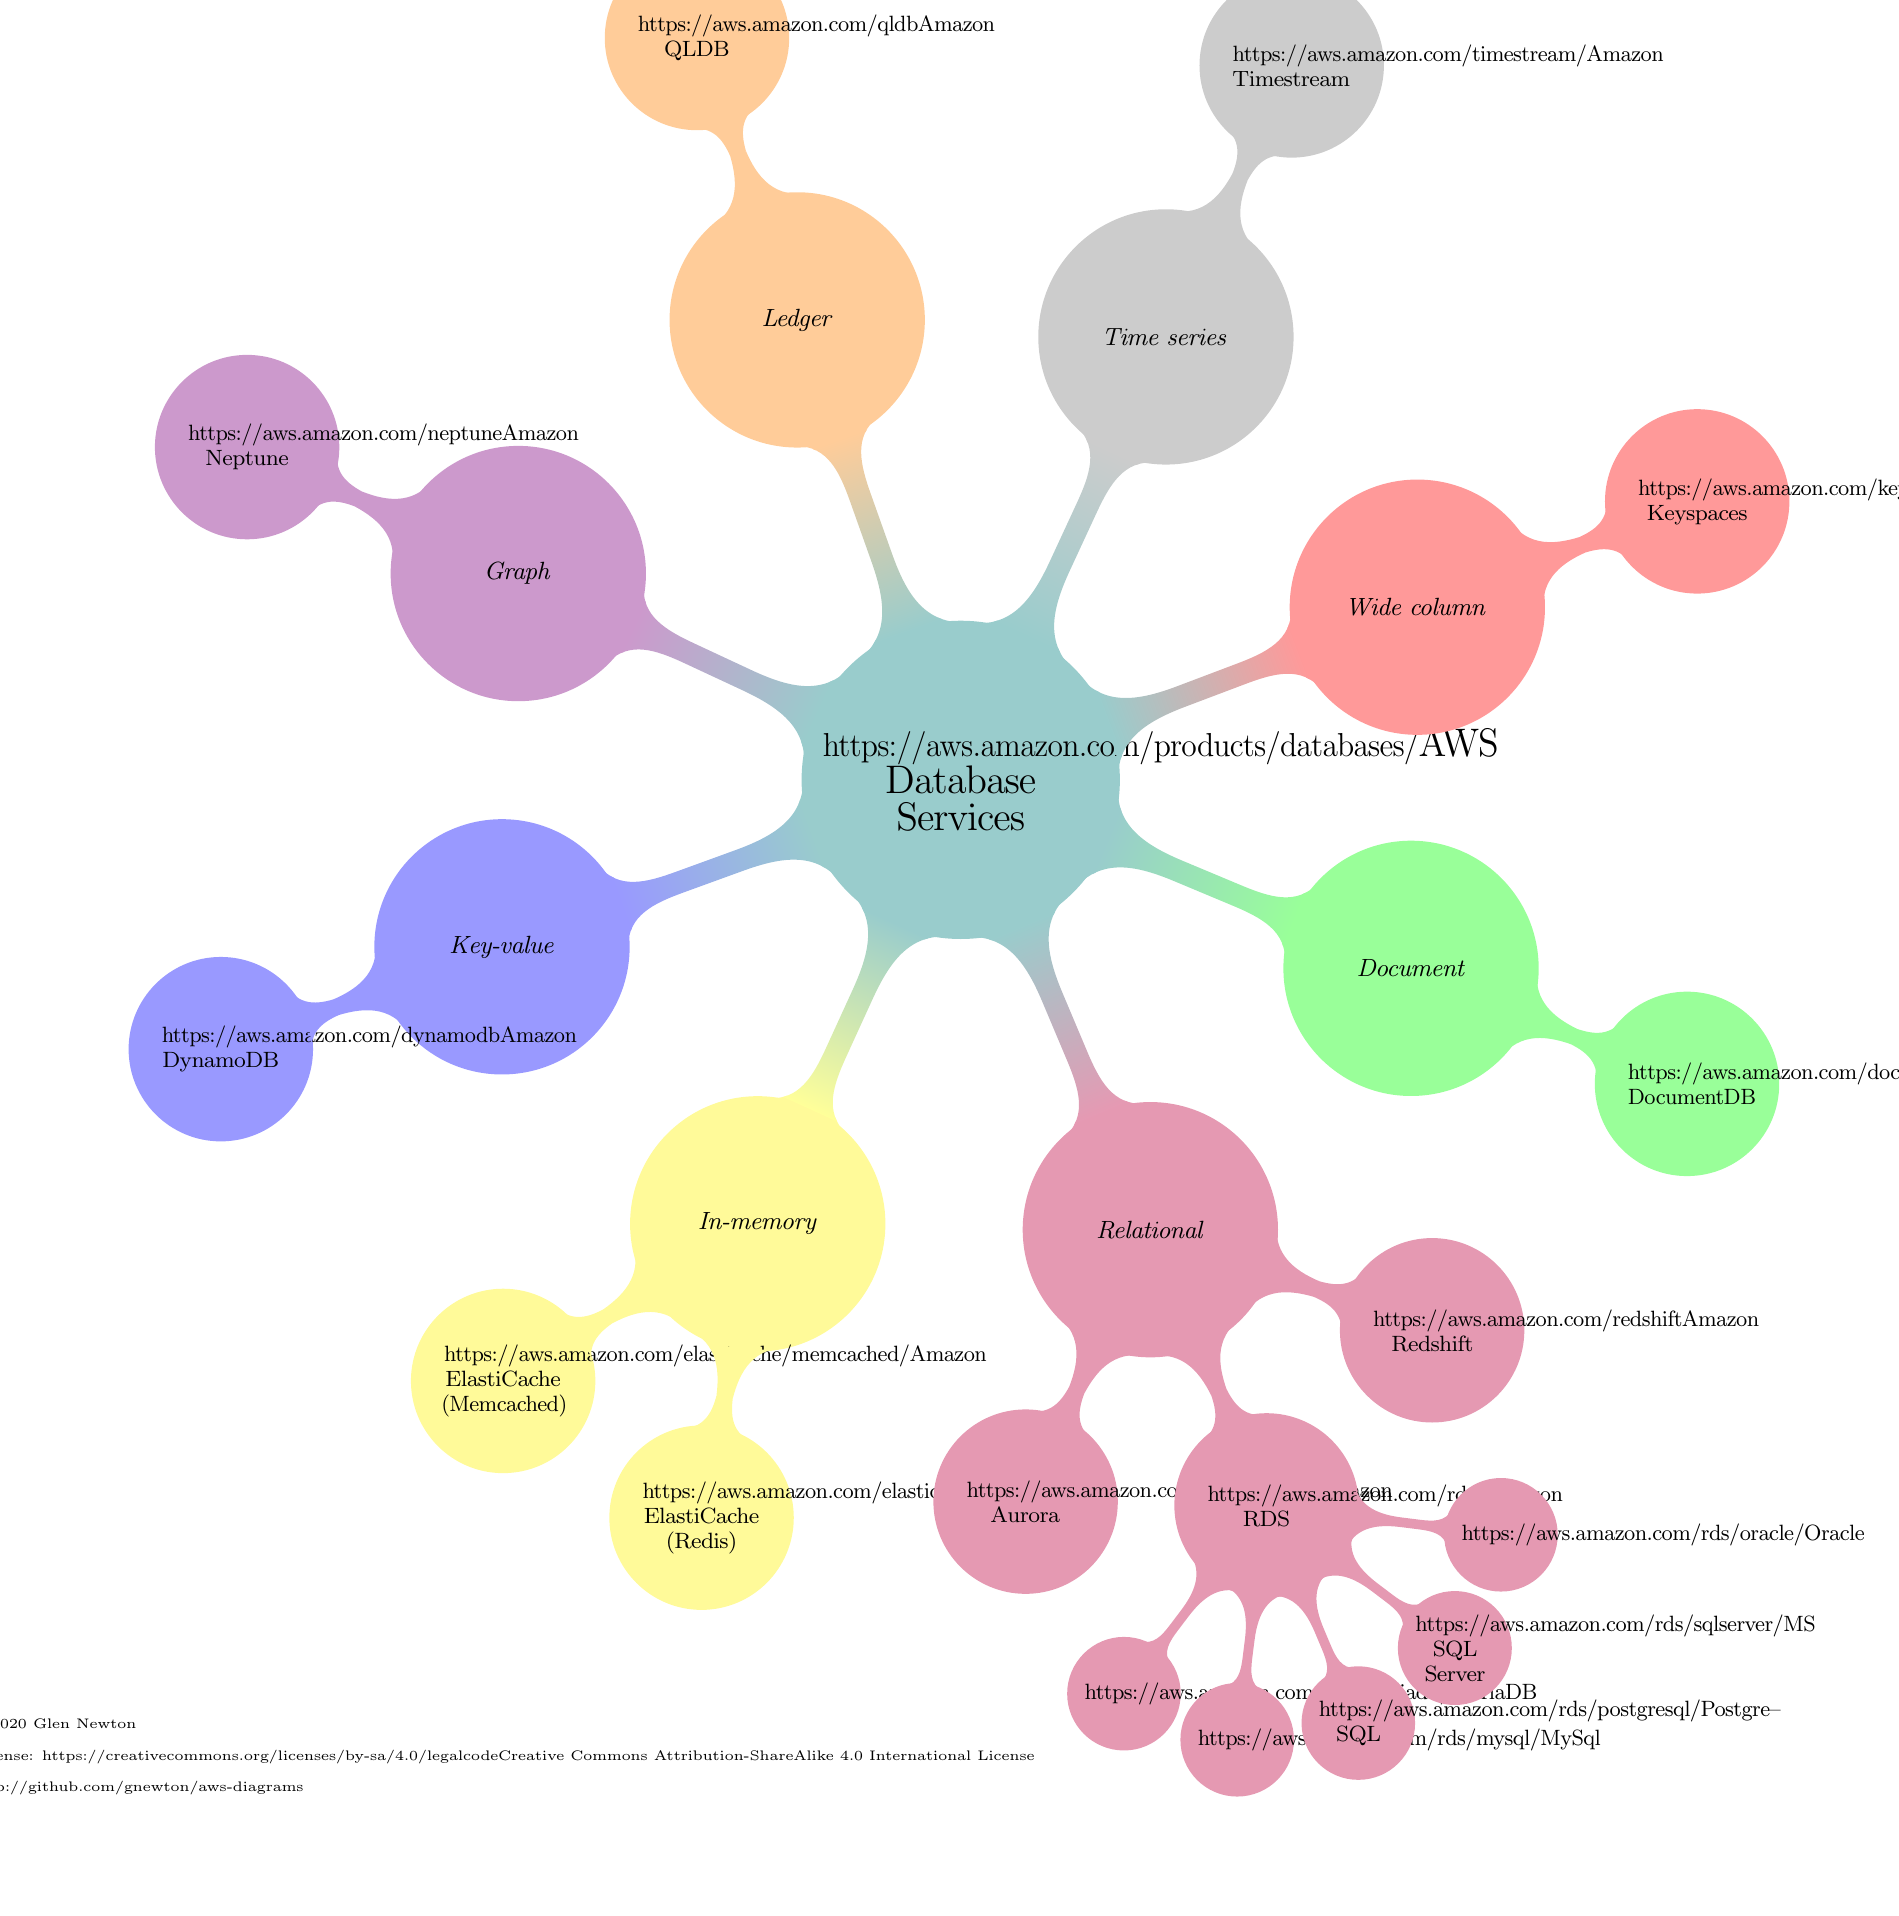
\begin{tikzpicture}
                \begin{scope}
                [mindmap,
                  grow cyclic,
                  every node/.style=concept,
                  concept color=teal!40,
                  level 1/.append style={sibling angle=360/7, level distance=6.2cm,minimum size=3.2cm},
                  level 2/.append style={sibling angle=37.5, level distance=3.8cm,minimum size=2.3cm},
                  level 3/.append style={level distance=3cm,minimum size=1.4cm,font=\footnotesize},
                ]
                \node [root concept] {\href{https://aws.amazon.com/products/databases/}{\Large AWS Database Services}}
                child [concept color=blue!40, rotate=20]{
                  node[concept] {\em Key-value}
                  child { node[concept] {\href{https://aws.amazon.com/dynamodb}{Amazon\\ DynamoDB}} }
                }
                child [concept color=yellow!40, rotate=14]{
                  node   {\em In-memory}%[clockwise from=45, level distance=8cm]
                  child [rotate=-15]{ node[concept,alias=foo] {\href{https://aws.amazon.com/elasticache/memcached/}{Amazon\\ ElastiCache\\ (Memcached)}} }
                  child [rotate=-5]{ node[concept] {\href{https://aws.amazon.com/elasticache/redis}{Amazon\\ ElastiCache\\ (Redis)}} }
                }
                child [concept color=purple!40, rotate=10]{
                  node    {\em Relational}
                  child [rotate=-10]{ node    {\href{https://aws.amazon.com/rds/aurora/}{Amazon Aurora}}}
                  child { node    {\href{https://aws.amazon.com/rds/}{Amazon RDS}}
                    child { node[concept] {\href{https://aws.amazon.com/rds/mariadb/}{MariaDB}} }
                    child { node[concept] {\href{https://aws.amazon.com/rds/mysql/}{MySql}} }
                    child { node[concept] {\href{https://aws.amazon.com/rds/postgresql/}{Postgre-- SQL} }}
                    child { node[concept] {\href{https://aws.amazon.com/rds/sqlserver/}{MS SQL Server} }}
                    child { node[concept] {\href{https://aws.amazon.com/rds/oracle/}{Oracle} }}
                  }
                  child [rotate=10] { node    {\href{https://aws.amazon.com/redshift}{Amazon Redshift}} }
                }
                child [concept color=green!40, rotate=3]{
                  node     {\em Document}
                  child { node    {\href{https://aws.amazon.com/documentdb}{Amazon\\ DocumentDB}} }
                }
                child [concept color=red!40, rotate=-5]{node  {\em Wide column}
                  child { node[concept] {\href{https://aws.amazon.com/keyspaces/}{Amazon Keyspaces}} }
                }
                child [concept color=gray!40, rotate=-12]{node  {\em Time series}
                  child { node[concept] {\href{https://aws.amazon.com/timestream/}{Amazon Timestream}} }
                }
                child [concept color=orange!40, rotate=-19] {node {\em Ledger}
                  child { node {\href{https://aws.amazon.com/qldb}{Amazon QLDB}} }
                }
                child [concept color=violet!40, rotate=-25] {node {\em Graph}
                  child { node {\href{https://aws.amazon.com/neptune}{Amazon Neptune}} }
                };
                \end{scope}
                \node[below=3cm of foo](foox) {
                  %                  Copyright 2020 Glen Newton
                                    \tiny
                  \begin{tabular}{l}
                    \copyright 2020 Glen Newton\\
                    \\
                    License: \href{https://creativecommons.org/licenses/by-sa/4.0/legalcode}{Creative Commons Attribution-ShareAlike 4.0 International License}\\
                    \\
                    \url{http://github.com/gnewton/aws-diagrams} \\
                  \end{tabular}

                };
            \end{tikzpicture}}\par}
          {\tiny

}
\end{document}
